\documentclass{article}

\usepackage[utf8]{inputenc}
\usepackage[T1]{fontenc}
\usepackage{amsmath}
\usepackage{xcolor} % Add this package for \textcolor
\usepackage{fancyhdr} % Add this package
\usepackage{ulem} % Add this package for better underlining
\usepackage{listings} % Add this package for code listings
\lstset{breaklines=true} % Enable line breaking in listings
\usepackage{graphicx} % Add this package for including images
\usepackage{hyperref}
\hypersetup{
    colorlinks=true,
    linkcolor=blue,
    citecolor=blue,
    filecolor=blue,
    urlcolor=blue,
    pdfborder={0 0 0}
}

\title{\LARGE\bfseries Comprehensive Data Science Documentation}
\author{
    \textbf{Prosenjit Mondol} \\
    \normalsize Data Scientist \\
    \normalsize \href{mailto:prosenjit1156@email.com}{prosenjit1156@email.com}
}
\date{\today}


\pagestyle{fancy} % Enable fancy header
\fancyhead[L]{My Personal Documentations} % Left side header with documentation name
\fancyhead[C]{} % Center header empty
\fancyhead[R]{Prosenjit} % Right side header empty
\renewcommand{\headrulewidth}{1pt} % Add a horizontal line under the header



\begin{document}

\maketitle

\tableofcontents % <-- Add this line for list view

\newpage % Start a new page after the table of contents

\section{Data Preprocessing}
\begin{itemize}
    \item \textbf{\textcolor{blue}{\dotuline{Sampling}}}\\
        Sampling techniques are used to select a representative subset of data from a large population to reduce the computational complexity and improve the efficiency of the analysis.
    \item \textbf{\textcolor{blue}{\dotuline{Transformation}}}\\
    Transformation techniques involve manipulating raw data to create a single input, such as scaling, normalization, or encoding categorical data.
    \item \textbf{\textcolor{blue}{\dotuline{Denoising}}}\\
    Denoising techniques remove unwanted noise from the data that can lead to inaccurate results.
    \item \textbf{\textcolor{blue}{\dotuline{Imputation}}}\\
    Imputation techniques are used to fill in missing values in the data using statistical methods.
    \item \textbf{\textcolor{blue}{\dotuline{Feature extraction}}}\\
    Feature extraction techniques help to identify and extract relevant features from the data that are significant in a particular context.
    \item \textbf{\textcolor{blue}{\dotuline{Normalization}}}\\
    Normalization techniques are used to organize data for more efficient access and processing.

\end{itemize}

\section{Handle Categorical Data}

Categorical data is a type of data that represents qualitative or nominal characteristics, such as gender, occupation, Categorical data cannot be measured or compared using mathematical operations like addition or subtraction.
\subsection{Different Encoding Methods for Categorical Data}
\begin{itemize}
    \item \textbf{\textcolor{blue}{\dotuline{One-Hot Encoding}}}\\
    One-Hot Encoding creates a new binary column for each category.
    \begin{lstlisting}[language=Python, caption={Logistic Regression Example}, label={lst:logreg}, backgroundcolor=\color{gray!10}, frame=single, keywordstyle=\color{blue}\bfseries, commentstyle=\color{green!50!black}, stringstyle=\color{orange}]
X = pd.get_dummies(X)
print(X)
    \end{lstlisting}
    \item \textbf{\textcolor{blue}{\dotuline{Label Encoding}}}\\
    Label Encoding assigns a numerical value to each category.
    \begin{center}
        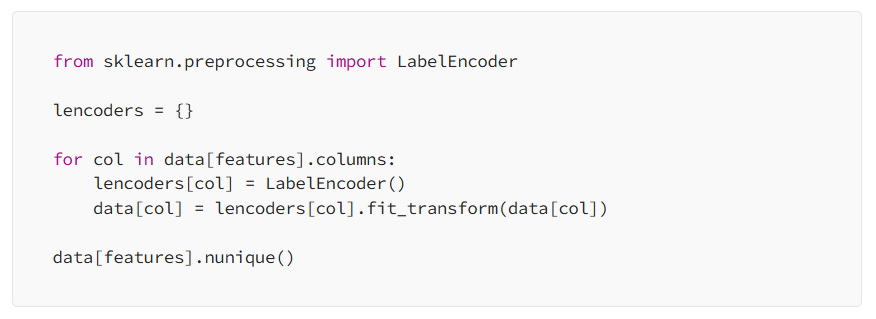
\includegraphics[width=0.5\textwidth]{label encoding} % Replace 'example-image' with your image filename (without extension)
    \end{center}
    \item \textbf{\textcolor{blue}{\dotuline{Binary Encoding}}}\\
    Binary Encoding creates new columns representing each category.
\end{itemize}

\subsection{Looking at null or missing values}
\begin{itemize}
    \item \textbf{\textcolor{blue}{\dotuline{Mean Imputation}}}\\
    Mean imputation is a simple and widely used method for filling in missing values. 
    \item \textbf{\textcolor{blue}{\dotuline{Mode Imputation}}}\\
    Mode imputation is a method for filling in missing values that is similar to mean imputation, but instead of using the mean, it uses the mode of the available values in a column.
    \item \textbf{\textcolor{blue}{\dotuline{K-Nearest Neighbor (KNN) Imputation}}}\\
    KNN imputation is a method for filling in missing values that is based on the distance between data poionts.
    \begin{center}
    \begin{lstlisting}[language=Python, caption={Logistic Regression Example}, label={lst:logreg}, backgroundcolor=\color{gray!10}, frame=single, keywordstyle=\color{blue}\bfseries, commentstyle=\color{green!50!black}, stringstyle=\color{orange}]
    # Multiple Imputation by Chained Equations
    from sklearn.experimental import enable_iterative_imputer
    from sklearn.impute import IterativeImputer

    #mputed_data = df[numerical_columns].copy(deep=True) 
    mice_imputer = IterativeImputer()
    data[numerical_columns] = mice_imputer.fit_transform(data[numerical_columns])
    \end{lstlisting}
    \end{center}
\end{itemize}

\section{Checking imblanced in target variable}
\begin{itemize}
    \item \textbf{\textcolor{blue}{\dotuline{Handling imbalanced data using oversampling}}}\\
    oversampling is a method for handling imbalanced data by increasing the size of the minority class.
    \begin{center}
    \begin{lstlisting}[language=Python, caption={Logistic Regression Example}, label={lst:logreg}, backgroundcolor=\color{gray!10}, frame=single, keywordstyle=\color{blue}\bfseries, commentstyle=\color{green!50!black}, stringstyle=\color{orange}]
from sklearn.utils import resample

no = normalized_data[normalized_data.RainTomorrow == 0]
yes = normalized_data[normalized_data.RainTomorrow == 1]
yes_oversampled = resample(yes, replace=True, n_samples=len(no), random_state=123)
oversampled_data = pd.concat([no, yes_oversampled])

fig = plt.figure(figsize = (8,5))
sns.countplot(x='RainTomorrow', data = oversampled_data, palette = "Set1").set(title='RainTomorrow Indicator No(0) and Yes(1) after Oversampling (Balanced Dataset)')
    \end{lstlisting}
    \end{center}
    
    \item \textbf{\textcolor{blue}{\dotuline{How multicollinearity affects decision trees}}}\\
    Multicollinearity affects decision trees by reducing the importance and accuracy of the input features.
    \begin{center}
    \begin{lstlisting}[language=Python, caption={Logistic Regression Example}, label={lst:logreg}, backgroundcolor=\color{gray!10}, frame=single, keywordstyle=\color{blue}\bfseries, commentstyle=\color{green!50!black}, stringstyle=\color{orange}]
    #the heat map of the correlation
    plt.figure(figsize=(16,10))
    sns.heatmap(X.corr(), annot=True, cmap='RdYlGn')
    \end{lstlisting}
    \end{center}
\end{itemize}

\section{Outliner Detection}
\begin{itemize}
    \item \textbf{\textcolor{blue}{\dotuline{Boxplot Method}}}\\
    One of the simplest and most popular methods for detecting outliers is the box-plot.
    \begin{center}
    \begin{lstlisting}[language=Python, caption={Logistic Regression Example}, label={lst:logreg}, backgroundcolor=\color{gray!10}, frame=single, keywordstyle=\color{blue}\bfseries, commentstyle=\color{green!50!black}, stringstyle=\color{orange}]
        plt.figure(figsize=(50,25))
        sns.boxplot(data=scaled_data[numerical_features])
    \end{lstlisting}
    \end{center}
    \item \textbf{\textcolor{blue}{\dotuline{Z-Score Method}}}\\
    The Z-Score method is a simple and widely used method for detecting outliers.
    \begin{center}
        \begin{lstlisting}[language=Python, caption={Logistic Regression Example}, label={lst:logreg}, backgroundcolor=\color{gray!10}, frame=single, keywordstyle=\color{blue}\bfseries, commentstyle=\color{green!50!black}, stringstyle=\color{orange}]
from scipy import stats
import numpy as np

# Calculate Z-scores for each value in the numerical features
z_scores = np.abs(stats.zscore(scaled_data[numerical_features]))

# Identify outliers (e.g., Z-score > 3)
outliers = (z_scores > 3)

# Print rows with outliers
print(scaled_data[outliers.any(axis=1)])
\end{lstlisting}
\end{center}
 \item \textbf{\textcolor{blue}{\dotuline{Transformation}}}\\
 Transformation involves transforming the data to a different scale to reduce the impact of the outliers.   
 \begin{center}
    \begin{lstlisting}[language=Python, caption={Logistic Regression Example}, label={lst:logreg}, backgroundcolor=\color{gray!10}, frame=single, keywordstyle=\color{blue}\bfseries, commentstyle=\color{green!50!black}, stringstyle=\color{orange}]
        from sklearn.preprocessing import PowerTransformer
        # Apply Power Transformation to the numerical features  
        power_transformer = PowerTransformer()
        scaled_data[numerical_features] = power_transformer.fit_transform(scaled_data[numerical_features])    
    \end{lstlisting}    
    \end{center}
\end{itemize}


\section{Let’s see how it fared in prediction using Logistic Regression}
\begin{center}
\begin{lstlisting}[language=Python, caption={Logistic Regression Example}, label={lst:logreg}, backgroundcolor=\color{gray!10}, frame=single, keywordstyle=\color{blue}\bfseries, commentstyle=\color{green!50!black}, stringstyle=\color{orange}]
# Train a logistic regression model on the training set
from sklearn.metrics import accuracy_score
from sklearn.linear_model import LogisticRegression

# Instantiate the model
logreg = LogisticRegression(solver='liblinear', random_state=0)

# Fit the model
logreg.fit(X_train, y_train)

# Predict on the test set
y_pred_test = logreg.predict(X_test)

print('Model accuracy score: {0:0.4f}'.format(accuracy_score(y_test, y_pred_test)))
\end{lstlisting}
\end{center}

\section{Models}
\subsection{Ensemble Model}
\noindent
\begin{center}
    \fcolorbox{blue}{blue!10}{
        \parbox{0.95\linewidth}{
            \textbf{Definition:} \\
            An ensemble model in machine learning combines the predictions of multiple individual models (base estimators) to produce a more accurate and robust prediction than any single model alone.
        }
    }
\end{center}

\subsection{SOTA Model}
\noindent
\begin{center}
    \fcolorbox{blue}{blue!10}{
        \parbox{0.95\linewidth}{
            \textbf{Definition:} \\
            In deep learning, SOTA model means State-of-the-Art model — basically, the best-performing architecture or method for a given task at a given time, according to benchmarks or competitions.
        }
    }
\end{center}




\end{document}
